\chapter{Om Kojo}
\begin{multicols}{2}
\section*{\color{black}Vad är Kojo?}
Kojo är en app som hjälper dig att lära dig att programmera. Med Kojo kan du koda i det moderna och kraftfulla programspråket {\bf\color{blue}Scala}. Kojo är gratis och finns på Svenska. Kojo fungerar med Linux, Windows och Mac OSX.
\section*{\color{black}Var hittar jag Kojo?}
Ladda ner Kojo här: 
\href{http://www.kogics.net/kojo-download}{www.kogics.net/kojo-download}
Läs mer här: 
\href{http://lth.se/programmera}{lth.se/programmera}

\columnbreak

\begin{center}
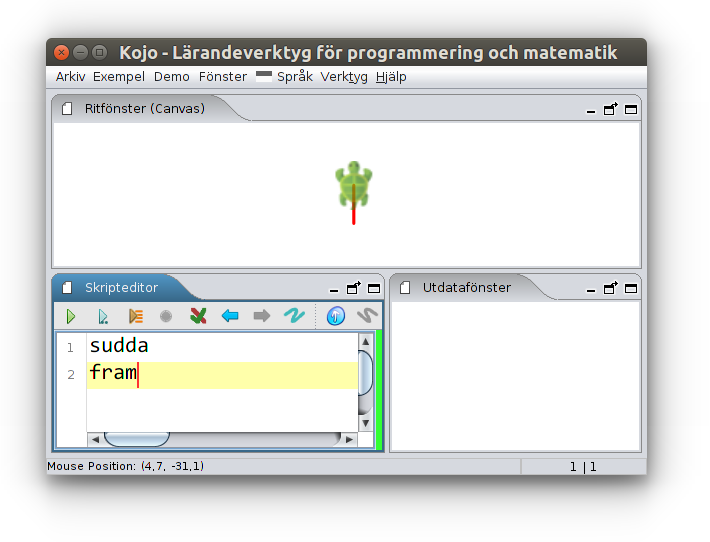
\includegraphics[width=14.0cm]{../img/kojo.png}
\end{center}

\end{multicols}

\chapter{Ditt första program}
\begin{multicols}{2}
\section*{\color{BrickRed}Uppdrag:}
Skriv så här i Kojos skripteditor-fönster:

\begin{lstlisting}[basicstyle={\ttfamily\fontsize{48.0}{48.0}\selectfont}]
sudda
fram
\end{lstlisting}
        
Tryck på den gröna play-knappen 

\includegraphics[width=1.0cm]{../img/play.png}
\\

för att köra igång ditt program.

\columnbreak

\begin{center}
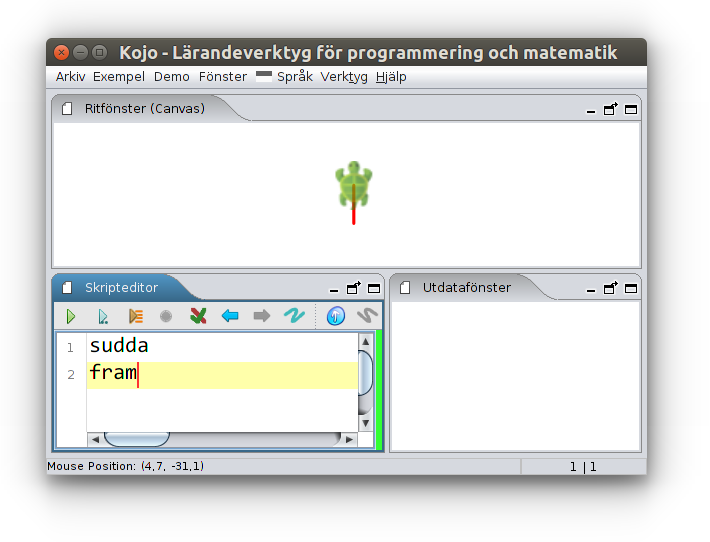
\includegraphics[width=14.0cm]{../img/fram.png}
\end{center}

\end{multicols}

\chapter{Rita en kvadrat}
\begin{multicols}{2}

\begin{lstlisting}[basicstyle={\ttfamily\fontsize{36.0}{36.0}\selectfont}]
sudda
fram
höger
\end{lstlisting}
        
Om du skriver \lstinline{vänster} eller \lstinline{höger} så vrider sig paddan.
\section*{\color{BrickRed}Uppdrag:}
Utöka programmet så att det blir en kvadrat.

\columnbreak

\begin{center}
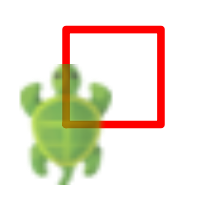
\includegraphics{../img/square.png}
\end{center}

\end{multicols}

\chapter{Rita en trappa}
\begin{multicols}{2}

\begin{lstlisting}[basicstyle={\ttfamily\fontsize{36.0}{36.0}\selectfont}]
sudda
fram; vänster
fram; höger
\end{lstlisting}
        
\vskip 1.0em
Med semikolon \lstinline{;} kan du ha flera satser på samma rad.
\section*{\color{BrickRed}Uppdrag:}
Utöka programmet så att det blir en trappa.

\columnbreak

\begin{center}

\includegraphics{../img/stairs.png}
\end{center}

\end{multicols}

\chapter{Gör en loop}
\begin{multicols}{2}

\begin{lstlisting}[basicstyle={\ttfamily\fontsize{36.0}{36.0}\selectfont}]
sudda
upprepa(4){fram; höger}
\end{lstlisting}
        
\section*{\color{BrickRed}Uppdrag:}


\begin{itemize}

\item {Vad händer om du ändrar 4 till 100?}
\item {Rita en trappa med 100 trappsteg.}

\end{itemize}



\columnbreak

\begin{center}
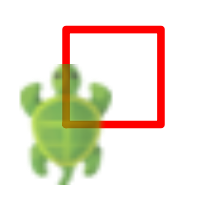
\includegraphics{../img/square.png}
\end{center}

\end{multicols}

\chapter{Rita en gubbe}
\begin{multicols}{2}
\section*{\color{BrickRed}Uppdrag:}
Rita en gubbe som du själv vill.
\section*{\color{OliveGreen}Tips:}

\begin{lstlisting}[basicstyle={\ttfamily\fontsize{24.0}{24.0}\selectfont}]
hoppa
vänster(180)
fram(300)
hoppa(100)
hoppaTill(25,-28)
skriv("FELIX är bäst")
\end{lstlisting}
        
Du kan se paddans läge nere till vänster medan du rör muspekaren i Ritfönstret:
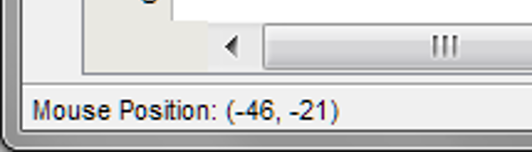
\includegraphics[width=6.0cm]{../img/mousepos.png}


\columnbreak


\begin{center}
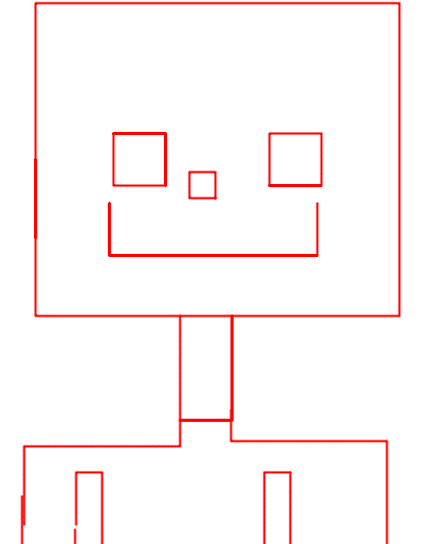
\includegraphics[width=4.5cm]{../img/man.png}
\end{center}

\vskip 2.0em
\begin{center}
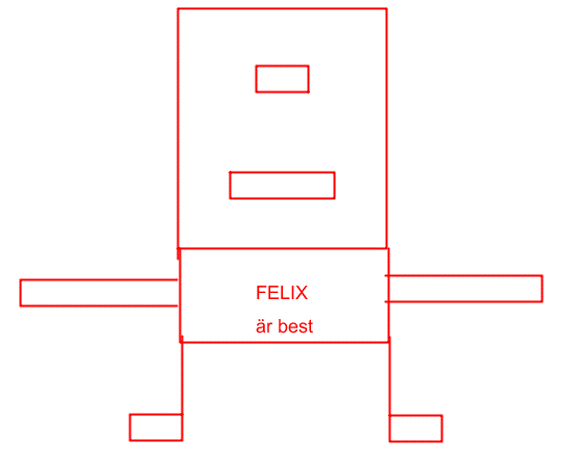
\includegraphics[width=9.0cm]{../img/alien.png}
\end{center}

\end{multicols}

\chapter{Gör din egen funktion}Med \lstinline{def} kan du göra egna {\it funktioner} som du själv väljer namn på.

\begin{lstlisting}[basicstyle={\ttfamily\fontsize{24.0}{24.0}\selectfont}]
def kvadrat =  upprepa(4){fram; höger}  

sudda
kvadrat    //använd din kvadrat-funktion
hoppa
kvadrat
\end{lstlisting}
        
\section*{\color{BrickRed}Uppdrag:}


\begin{itemize}

\item {Byt färg på kvadraterna.}
\item {Gör fler kvadrater.}

\end{itemize}


\section*{\color{OliveGreen}Tips:}

\begin{lstlisting}
fyll(grön); färg(lila)
\end{lstlisting}
        
\chapter{Stapla kvadrater}
\begin{multicols}{2}
\section*{\color{BrickRed}Uppdrag:}
Gör en stapel med 10 kvadrater.
\section*{\color{OliveGreen}Tips:}
Använd \lstinline{kvadrat} och \lstinline{hoppa} inuti en loop:
\vskip 1.0em

\begin{lstlisting}
def kvadrat =  upprepa(4){fram; höger}  

sudda; sakta(100)
upprepa(10){ ??? }
\end{lstlisting}
        

\columnbreak

\begin{center}
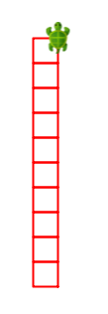
\includegraphics{../img/square-column.png}
\end{center}

\end{multicols}

\chapter{Gör en stapelfunktion}
\begin{multicols}{2}
\section*{\color{BrickRed}Uppdrag:}
Gör en funktion som heter \lstinline{stapel}, som ritar en stapel med 10 kvadrater.
\section*{\color{OliveGreen}Tips:}

\begin{lstlisting}
def kvadrat = upprepa(4){fram; höger}  
def stapel = ???

sudda; sakta(100)
stapel
\end{lstlisting}
        

\columnbreak

\begin{center}
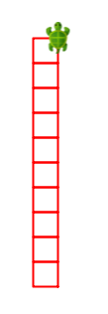
\includegraphics{../img/square-column.png}
\end{center}

\end{multicols}

\chapter{Gör ett rutnät}
\begin{multicols}{2}
\section*{\color{BrickRed}Uppdrag:}
Gör rutnät med 10*10 kvadrater.
\section*{\color{OliveGreen}Tips:}


\begin{itemize}

\item {Använd din stapelfunktion från tidigare.}
\item {Du kan hoppa baklänges en hel stapelhöjd med \lstinline{hoppa(-10*25)}}
\item {Du kan sedan hoppa till rätt plats med \lstinline{höger; hoppa; vänster}}

\end{itemize}



\columnbreak

\begin{center}
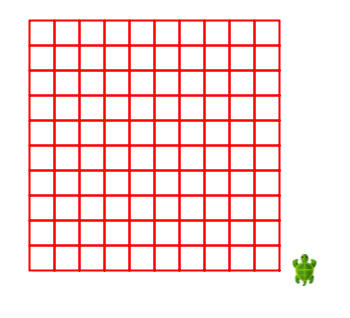
\includegraphics{../img/square-grid.png}
\end{center}

\end{multicols}

\chapter{Funktion med parameter}
\begin{multicols}{2}
Med en {\it parameter} kan funktioner göra olika saker:

\begin{lstlisting}
def kvadrat(sidlängd : Heltal) = 
  upprepa(4){fram(sidlängd); höger}

sudda; sakta(100); osynlig
kvadrat(100) 
kvadrat(70)
kvadrat(40)
\end{lstlisting}
        
\section*{\color{BrickRed}Uppdrag:}
Rita olika stora kvadrater med olika färg.
\section*{\color{OliveGreen}Tips:}

\begin{lstlisting}
fyll(blå); färg(rosa)
\end{lstlisting}
        


\columnbreak


\begin{center}
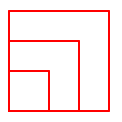
\includegraphics[width=10.0cm]{../img/square-param.png}
\end{center}

\end{multicols}

